\documentclass[11pt,a4paper]{article}
\renewcommand{\familydefault}{\sfdefault}
\usepackage{graphicx}
\usepackage{float}
\usepackage{geometry}
\usepackage{amsmath}

 \geometry{
 a4paper,
 left=0.63in,
 right=0.63in,
 top=0.8in,
 bottom=1in
 }
\graphicspath{ {graphics/} }

\begin{document}


%% Title
\begin{titlepage}
	\title{PrEP Dynamic Deterministic Compartmental Model}
	\date{\today}
	\author{Allen Roberts}
\end{titlepage}
\maketitle

%% Table of contents
\tableofcontents

%% Overview
\section{Overview}
This dynamic deterministic compartmental model evaluates the effect of pre-exposure prophylaxis (PrEP) rollout in a generalized HIV epidemic setting. The system of ordinary differential equations (ODEs) specified by the model are solved using Euler integration using a time step of 0.01 years. The model is written in \textbf{R}. 

The model simulates an HIV epidemic from 1980 to 2030. The population is stratified according to age, sex, and behavioral risk group and captures demographic, behavioral, and clinical dynamics. HIV-negative individuals experience aging, fertility, and mortality. HIV infection occurs due to sexual mixing between males and females across age and risk groups. Upon HIV infection, individuals enter a transient acute infection stage characterized by high viremia followed by progression through four CD4 count categories. The model allows HIV-negative persons to initiate and discontinue PrEP, HIV-positive persons to initiate and discontinue antiretroviral therapy (ART), and males to become circumcised either at birth or in adulthood. All members begin initially uninfected. In the first time-step, 0.1\% of the population is seeded with HIV infection. 

%% State variables
\section{State variables}
State variables are indicated as $X_{d,k,p}^{a,s,r}$, where:

\begin{itemize}
\item $a$ refers to age group, where $a = 1$ for ages 0 to 4; $a = 2$ for ages 5-9; ... ; $a = 12$ for ages 55-59.
\item $s$ refers to sex and circumcision status, where $s = 1$ refers to females, $s = 2$ refers to uncircumcised males, and $s = 3$ refers to circumcised males
\item $r$ refers to behavioral risk group, where $r = 1$ indicates low risk for HIV infection, $r = 2$ indicates medium risk, and $r = 3$ indicates high risk.
\item $d$ refers to HIV status, where $d = 1$ indicates susceptible, $d = 2$ indicates acute HIV, $d = 3$ indicates CD4 $>$500, $d = 4$ indicates CD4 350-499, $d = 5$ indicates CD4 200-349, and $d = 6$ indicates CD4 $<$200.
\item $k$ indicates treatment status, where $k = 1$ indicates not on ART and $k = 2$ indicates taking ART.
\item $p$ indicates PrEP status, where $p = 1$ indicates not on PrEP and $p = 2$ indicates taking PrEP.
\end{itemize}

\section{Parameters}
\begin{itemize}
\item $\mu_{d}^{a,s = 1}$ refers to the fertility rate.
\item $\nu^{a,s}$ refers to the background (non-HIV) mortality rate.
\item $\alpha_{d}^{a,s}$ refers to the HIV-associated mortality rate.
\item $\lambda_{d = 1,k = 1,p}^{a,s,r}$ refers to the force of infection experienced by HIV-negative individuals. 
\item $\sigma_{d}$ refers to the HIV disease progression rate.
\item $\theta_{d, k = 1}^{a,s,r}$ refers to the ART initiation rate
\item $\gamma_{d, k = 2}^{a,s,r}$ refers to the ART dropout rate
\item $\phi_{d = 1, k = 1}^{a,s,r}$ refers to the PrEP initiation rate
\item $\zeta_{d = 1, k = 1}^{a,s,r}$ refers to the PrEP dropout rate
\item $\tau$ refers to the risk of HIV infection among PrEP users relative to those among PrEP non-users.
\end{itemize}

\section{Model structure}
\begin{figure}[H]
\centering
\caption{Structure of dynamic deterministic model}
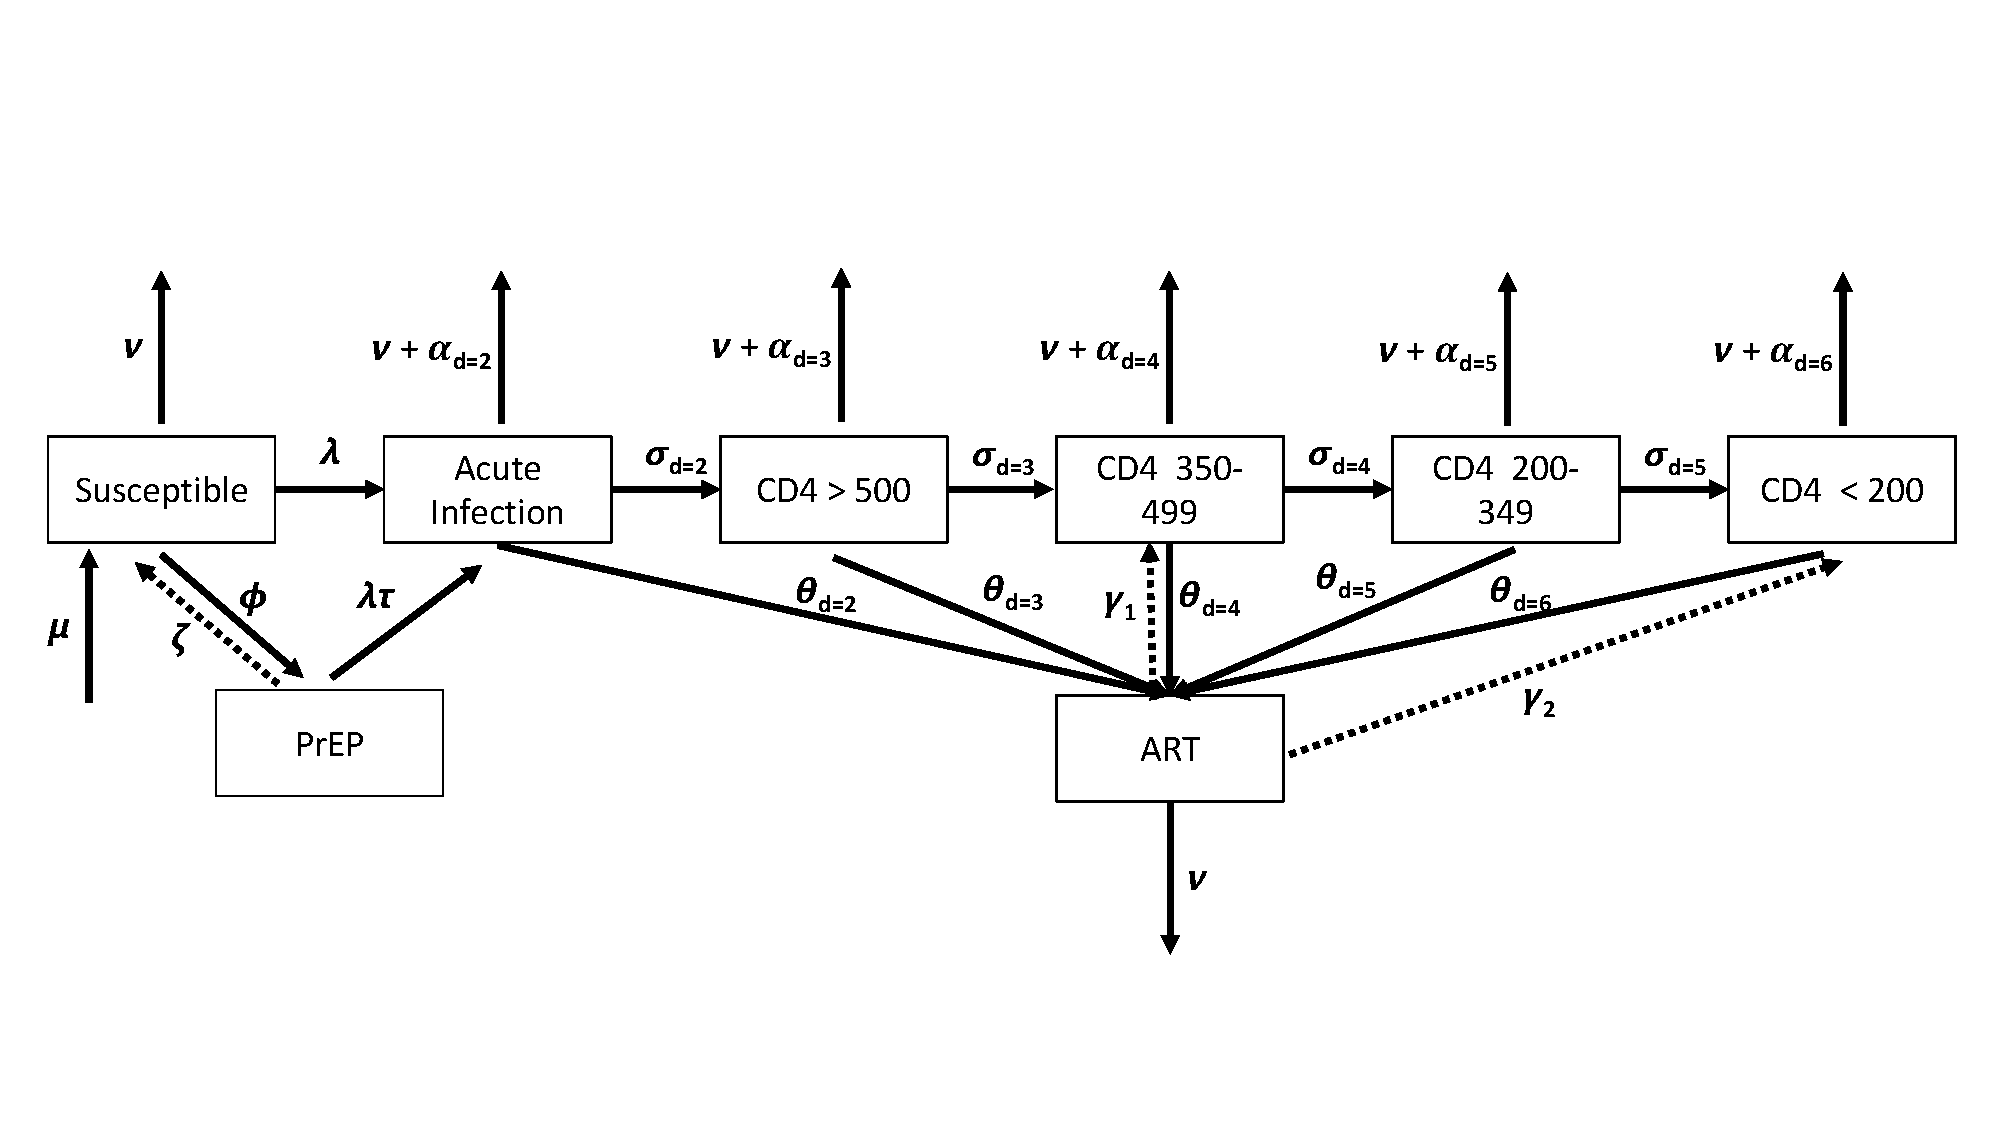
\includegraphics[width = 175mm]{prep-dc2m-diagram.pdf}
\end{figure}

\section{Model equations}

\section{Disease progression}
Newly-infected individuals enter a transient acute infection phase characterized by asymptomatic high viremia. They then progress through four CD4 stages ($\geq$ 500, 350-499, 200-349, and $\leq$ 200). Viral load is assumed to be high during acute infection and then constant across CD4 counts.

\section{Demography}
	\subsection{Aging}
	As each compartment is indexed to a five-year age group, one-fifth of each compartment progresses to the next age group each year. Individuals entering the older age group are redistributed to match the assumed sexual risk profile of the new age group. Population influx occurs through births into the 0-4 age group, while individuals who age out of the 55-59 age group exit the population. Therefore, each state has an ODE corresponding to aging that occurs at each time step.

	\[
			dX_{d,k,p}^{a,s,r}(t) =
		\begin{cases}
			-\frac{t}{5}X_{d,k,p}^{a,s,r}(t), & \text{if } a=0\\
			-\frac{t}{5}X_{d,k,p}^{a,s,r}(t) + \frac{t}{5}\sum\limits_{r=1}^3 X_{d,k,p}^{a,s,r}, & \text{if } a\neq0
		\end{cases}
	\]

	\subsection{Mortality}
	Individuals can exit the population through HIV-specific or non-HIV mortality. HIV-specific mortality rates are dependent on both age and CD4 count. Individuals in the youngest (0-4) and oldest (55-59) age groups experience higher HIV-specific mortality rates as shown below:	


	\subsection{Fertility}




\section{Interventions}

\section{Behavioral risk}

\section{Transmission}


\section{Initial conditions}

\section{Model fitting}

\section{Uncertainty analysis}

\section{Scenarios}

\section{Discussion}

\section{References}


\end{document}
